\documentclass[11pt,a4paper]{article}

\usepackage[T1]{fontenc}
\usepackage[utf8]{inputenc}
\usepackage{lmodern}
\usepackage{geometry}
\usepackage{amsmath,amssymb}
\usepackage{booktabs}
\usepackage{graphicx}
\usepackage{xcolor}
\usepackage{hyperref}
\usepackage{caption}

\geometry{margin=1in}
\graphicspath{{./}{../experiments/local_occurrence_execution_paper73/}}
\hypersetup{
  colorlinks=true,
  linkcolor=blue!60!black,
  citecolor=blue!60!black,
  urlcolor=blue!60!black
}

\newcommand{\Lstar}{L_\star}
\newcommand{\Ggate}{G_{\rm gate}}
\newcommand{\Glocal}{G_{\rm gate+L}}
\newcommand{\Rrob}{R_{\rm rob}}

\title{\textbf{Execution of the Local Occurrence Hypothesis}\\
\large Paper 73 --- First Test of the Preregistered SAT-Specific Protocol}
\author{Christof Krieg\\
\small Independent Researcher\\
\small MAAT Structural Selection Project}
\date{2026}

\begin{document}
\maketitle

\begin{abstract}
Paper 72 preregistered a SAT-specific follow-up to Gate Challenge Cycle I:
the Local Occurrence Hypothesis. The hypothesis stated that decision-local
occurrence/degree residuals might add useful SAT branching information beyond
the frozen MAAT v1.7 gate. This paper executes that frozen protocol without
changing the definition of $\Lstar$, the residualization rule, calibration
splits, budgets, bootstrap procedure, baselines, or interpretation criteria.

The dataset gatekeeper passed on 55 public SATLIB/DIMACS benchmark instances
with SHA256-verified manifests and parseable DIMACS files. The execution used
11 calibration instances and 44 test instances across six benchmark families.
Under the preregistered interpretation rule, Gate+L failed to beat the frozen
gate with a positive 95\% confidence lower bound
($\Delta=-13.2382$, CI $[-37.3121,6.0309]$), failed to beat score-with-R
robustly ($\Delta=6.3392$, CI $[-8.5437,21.7627]$), and failed the
shuffled-$L$ null test ($\Delta=-6.8162$, CI $[-20.1598,6.0438]$). It also
lost clearly against MOMS ($\Delta=-84.9530$, CI $[-130.0199,-44.5361]$).

Under the preregistered interpretation criteria, the Local Occurrence
Hypothesis receives \texttt{no\_minimum\_support}. Paper 72 remains the
preregistered protocol document. Paper 73 reports only that the frozen
hypothesis did not pass its first execution test.
\end{abstract}

\section{Purpose and Guardrails}

Gate Challenge Cycle I produced a negative external SAT/CDCL result for the
frozen MAAT v1.7 gate and motivated a diagnostic question: did the gate miss a
decision-local occurrence or degree channel? Paper 72 converted that question
into a preregistered hypothesis and explicitly froze the next test before any
new Gate+L execution. The cycle archive is recorded in the Research Series II
release \cite{seriesii}.

This paper is an execution report. It does not introduce a new MAAT version,
does not alter the Paper-68 gate, and does not modify the Paper-72 local
channel. In particular, it does not tune thresholds, change residualization,
adjust weights, redesign the solver policy, or reinterpret the success
criteria after seeing the result.

The only allowed interpretation classes are those declared in Paper 72:
\[
\texttt{no\_minimum\_support},\qquad
\texttt{minimum\_support\_only},\qquad
\texttt{strong\_sat\_support}.
\]

\section{Frozen Protocol}

The Paper-72 hypothesis introduced a SAT-specific local residual coordinate
$\Lstar$ derived from occurrence and degree channels after calibration-only
residualization against the frozen structural coordinates. In the execution
code, the frozen channel is
\begin{equation}
  \Lstar(F)
  =
  \frac{1}{2}\left[z(D_{\rm res})-z(O_{\rm res})\right],
  \label{eq:lstar}
\end{equation}
where $O_{\rm res}$ and $D_{\rm res}$ are the residualized occurrence and
degree terms, and the $z$-standardization is performed using calibration-fold
statistics only. This definition is reported here for reproducibility; it is
not changed in Paper 73.

The frozen Gate+L wrapper is
\begin{equation}
  \Glocal(F)
  =
  \sigma\!\left(
    \operatorname{logit}(\Ggate(F))+\Lstar(F)
  \right),
  \label{eq:gateplusl}
\end{equation}
with no free multiplier on $\Lstar$. This deliberately prevents the execution
paper from becoming a hyperparameter search.

\section{Data, Licensing, and Reproducibility}

The external benchmark source is SATLIB, accessed through the public SATLIB
benchmark page \cite{satlib}. The benchmark page provides DIMACS CNF instances
and lists the benchmark families used here, but it does not present an explicit
open data license for raw redistribution. For that reason, the repository
version of this experiment intentionally excludes raw CNF files and downloaded
SATLIB archives.
SATLIB benchmark instances are not redistributed in this repository or release.
The included manifests contain only source URLs, hashes, and metadata required
for reproducibility. Users must obtain the original benchmark instances from
SATLIB and cite the SATLIB source.

\begin{table}[h]
\centering
\caption{Repository data-policy audit for Paper 73.}
\begin{tabular}{lll}
\toprule
Artifact & Repository status & License/data note \\
\midrule
Raw SATLIB CNFs & Excluded & Must be obtained from SATLIB \\
SATLIB archives & Excluded & Not redistributed \\
Manifest CSV & Included & URLs, hashes, metadata only \\
Solver CSV/JSON & Included & Derived outputs generated by this run \\
Figures & Included & Generated from derived outputs \\
Code and README & Included & Project-owned experiment scaffold \\
\bottomrule
\end{tabular}
\end{table}

The data gatekeeper verifies manifest completeness, file existence, SHA256
hashes, DIMACS parseability, and absence of unexpected CNF files before solver
execution. The executed dataset passed all checks:
\begin{table}[h]
\centering
\caption{Dataset gatekeeper result.}
\begin{tabular}{lr}
\toprule
Check & Result \\
\midrule
Manifest & PASS \\
CNFs present & PASS \\
SHA256 verification & PASS \\
DIMACS parseability & PASS \\
Unexpected files & PASS \\
Dataset ready & YES \\
\bottomrule
\end{tabular}
\end{table}

The run used 55 SATLIB/DIMACS instances: 10 AIM, 10 Dubois, 5 pigeon-hole,
10 flat graph-colouring, 10 UF20-91, and 10 UUF50-218 instances. The frozen
split contained 11 calibration instances and 44 test instances.

\section{Policies and Metrics}

The execution compared the following policies, including a VSIDS-style CDCL
baseline following the Chaff tradition \cite{chaff} and the classical
Jeroslow--Wang rule \cite{jeroslow-wang}:
\[
\{\text{VSIDS},\ \text{MOMS},\ \text{Jeroslow--Wang},\
\text{score-with-R},\ \text{frozen gate v1.7},\ \text{Gate+L},\
\text{Gate+shuffled-L}\}.
\]

The conflict budget was 5000 and the runtime budget was 30 seconds. Confidence
intervals were computed by paired bootstrap with 10000 resamples and seed
72072. For a comparator $C$, the reported paired utility delta is
\[
  \Delta(C,\text{Gate+L})
  =
  \operatorname{cost}(C)-\operatorname{cost}(\text{Gate+L}).
\]
Thus positive $\Delta$ means Gate+L required lower compute cost than the
comparator; negative $\Delta$ means Gate+L was worse.

\section{Results}

\begin{table}[h]
\centering
\small
\setlength{\tabcolsep}{4pt}
\caption{Primary paired comparisons on the 44-instance test split. Positive
$\Delta$ means Gate+L is better.}
\begin{tabular}{lrrrrr}
\toprule
Comparison & Mean $\Delta$ & CI low & CI high & Gate+L wins & Gate+L losses \\
\midrule
Gate+L vs frozen gate v1.7 & -13.2382 & -37.3121 & 6.0309 & 20 & 22 \\
Gate+L vs score-with-R & 6.3392 & -8.5437 & 21.7627 & 22 & 20 \\
Gate+L vs MOMS & -84.9530 & -130.0199 & -44.5361 & 5 & 37 \\
Gate+L vs Jeroslow--Wang & -106.8685 & -400.5297 & 64.2660 & 15 & 27 \\
Gate+L vs VSIDS & -384.7766 & -973.2246 & 6.0257 & 18 & 25 \\
Gate+L vs shuffled-L & -6.8162 & -20.1598 & 6.0438 & 21 & 23 \\
\bottomrule
\end{tabular}
\end{table}

The minimum-support rule required Gate+L to beat both frozen gate v1.7 and
score-with-R with positive 95\% confidence lower bounds, and to survive the
shuffled-$L$ null. None of these three conditions was met. The strong-SAT
support rule additionally required positive confidence lower bounds against
MOMS and Jeroslow--Wang; these conditions were also not met.

\begin{table}[h]
\centering
\caption{Policy-level compute-cost summary on the test split.}
\begin{tabular}{lrrrr}
\toprule
Policy & Mean cost & Median cost & Solve rate & Timeout rate \\
\midrule
VSIDS & 406.7354 & 50.8760 & 0.9773 & 0.0227 \\
MOMS & 706.5590 & 29.7320 & 0.9318 & 0.0682 \\
Jeroslow--Wang & 684.6435 & 33.9140 & 0.9545 & 0.0455 \\
score-with-R & 797.8512 & 53.6500 & 0.9318 & 0.0682 \\
frozen gate v1.7 & 778.2738 & 55.4080 & 0.9318 & 0.0682 \\
Gate+L & 791.5120 & 48.8220 & 0.9318 & 0.0682 \\
Gate+shuffled-L & 784.6958 & 50.6620 & 0.9318 & 0.0682 \\
\bottomrule
\end{tabular}
\end{table}

\section{Figures}

The generated figures are included for auditability and visual inspection.
They are derived from the committed CSV outputs and contain no raw DIMACS
clauses.

\begin{figure}[h]
\centering

\includegraphics[width=0.90\linewidth]{outputs_paper73_local_occurrence_execution/fig1_policy_compute_cost.png}
\caption{Median compute cost by policy on the test split.}
\end{figure}

\begin{figure}[h]
\centering
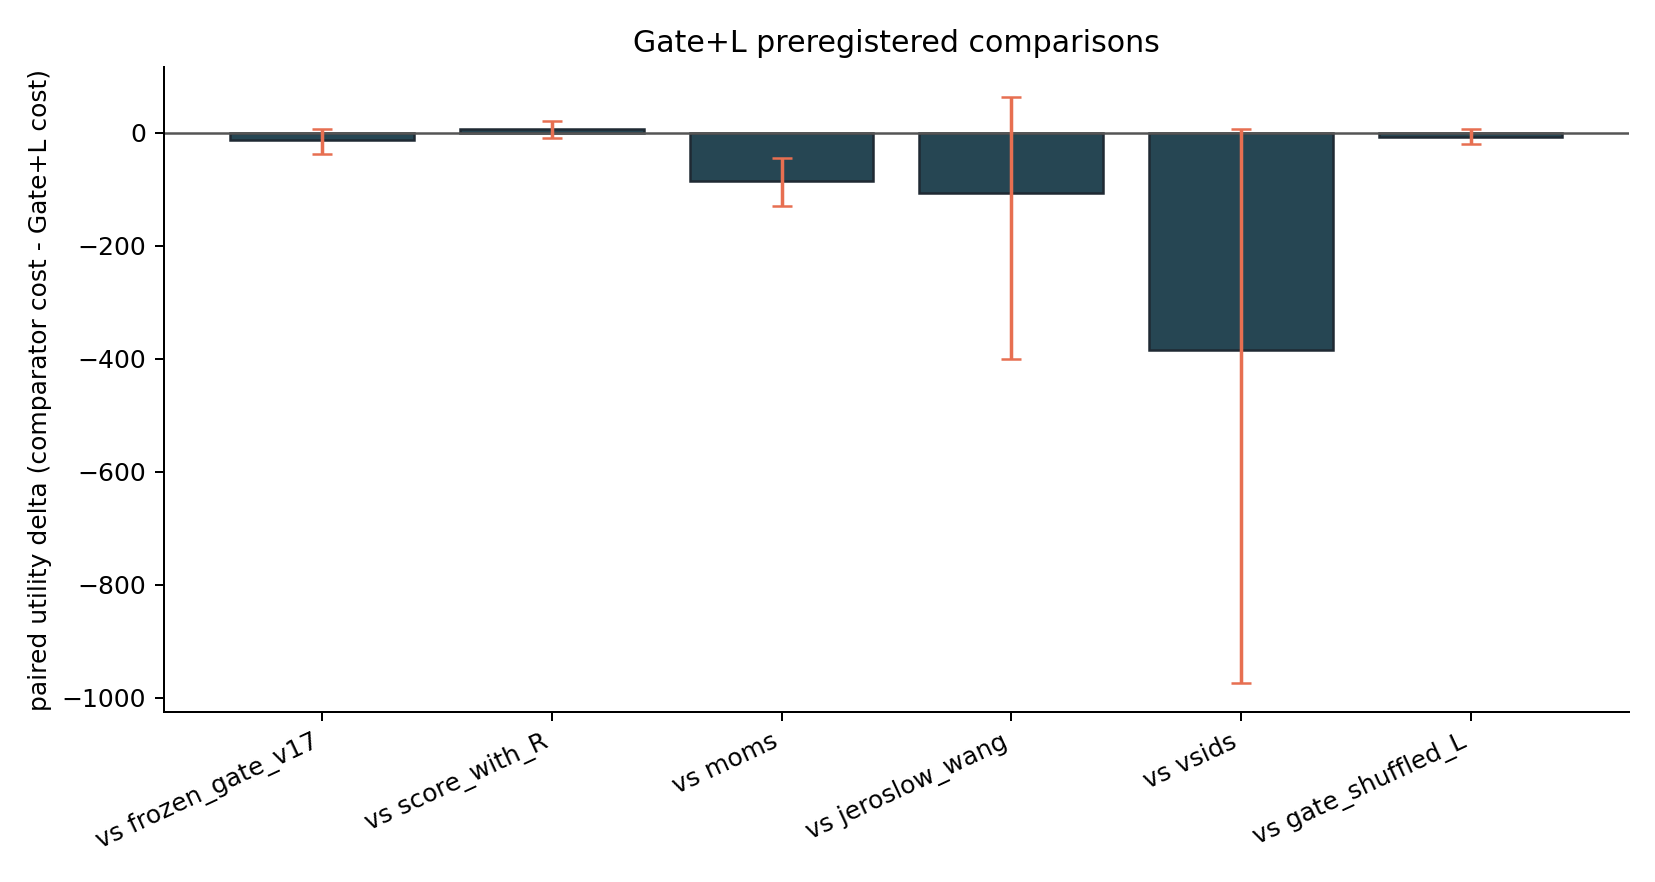
\includegraphics[width=0.90\linewidth]{outputs_paper73_local_occurrence_execution/fig2_gate_l_comparisons.png}
\caption{Paired Gate+L comparisons with bootstrap confidence intervals.}
\end{figure}

\begin{figure}[h]
\centering
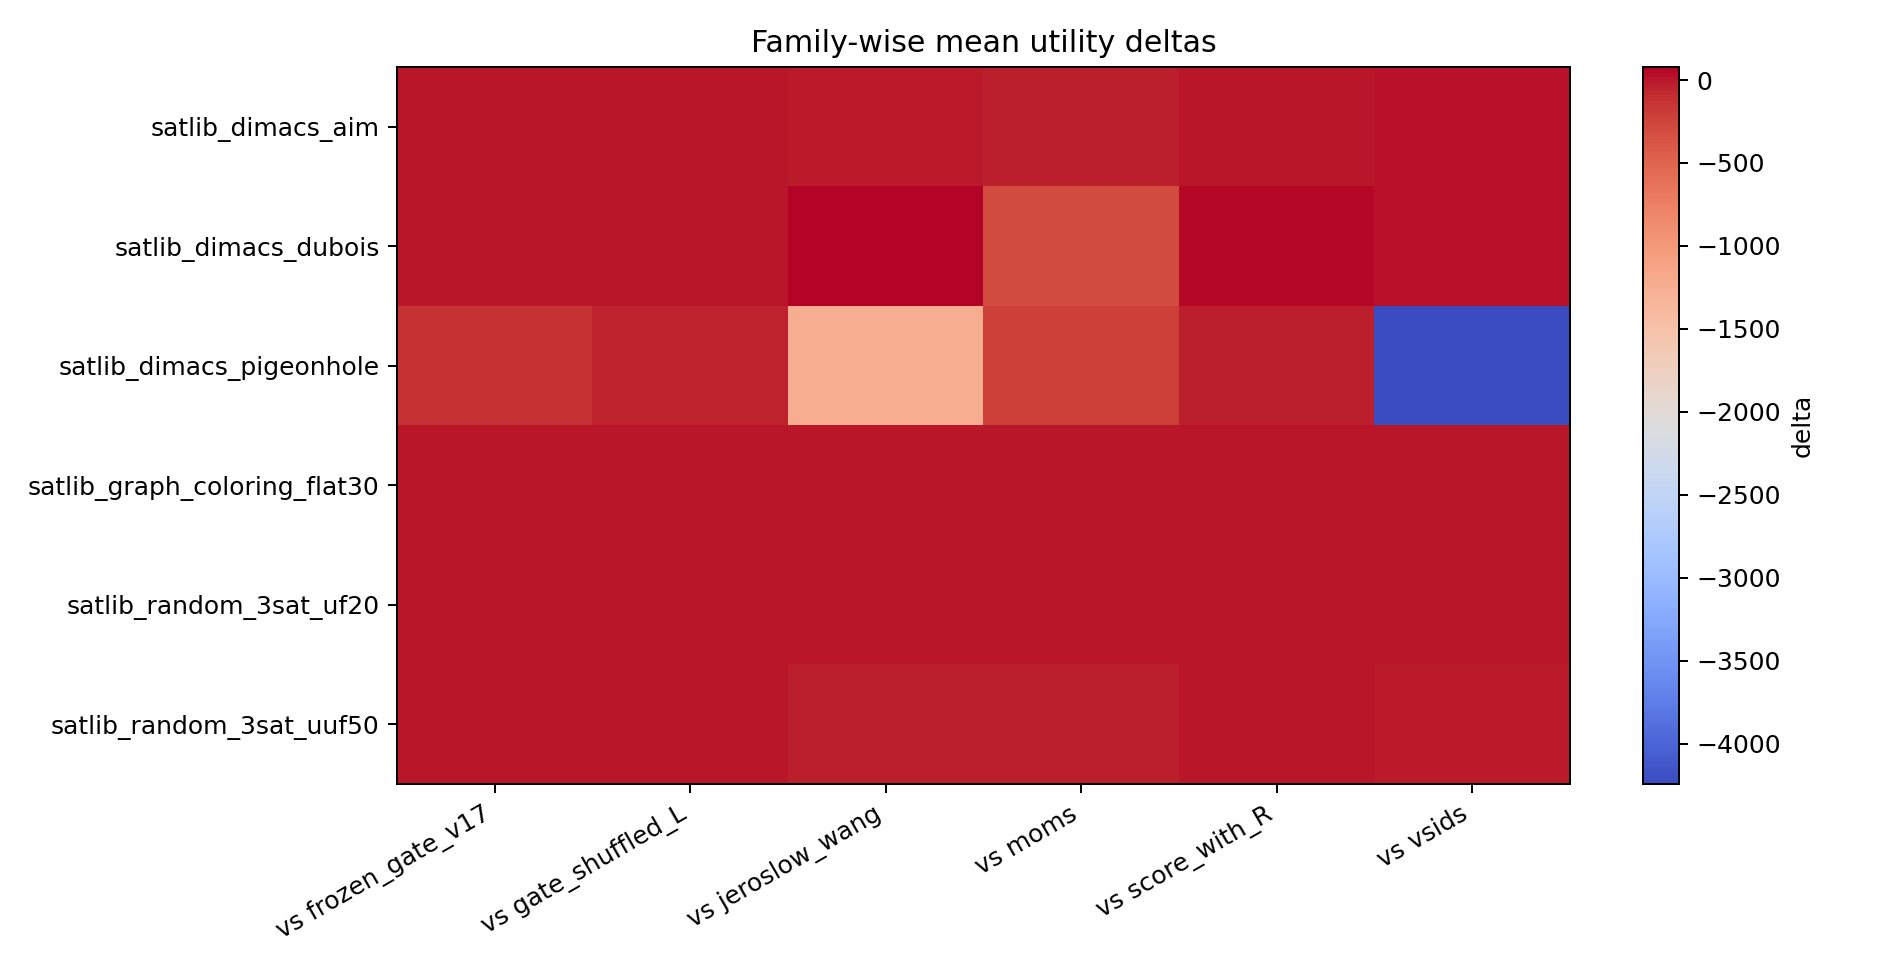
\includegraphics[width=0.90\linewidth]{outputs_paper73_local_occurrence_execution/fig3_family_delta_heatmap.png}
\caption{Family-level paired utility deltas. The strongest negative effects
are concentrated in pigeon-hole and classical heuristic comparisons.}
\end{figure}

\begin{figure}[h]
\centering
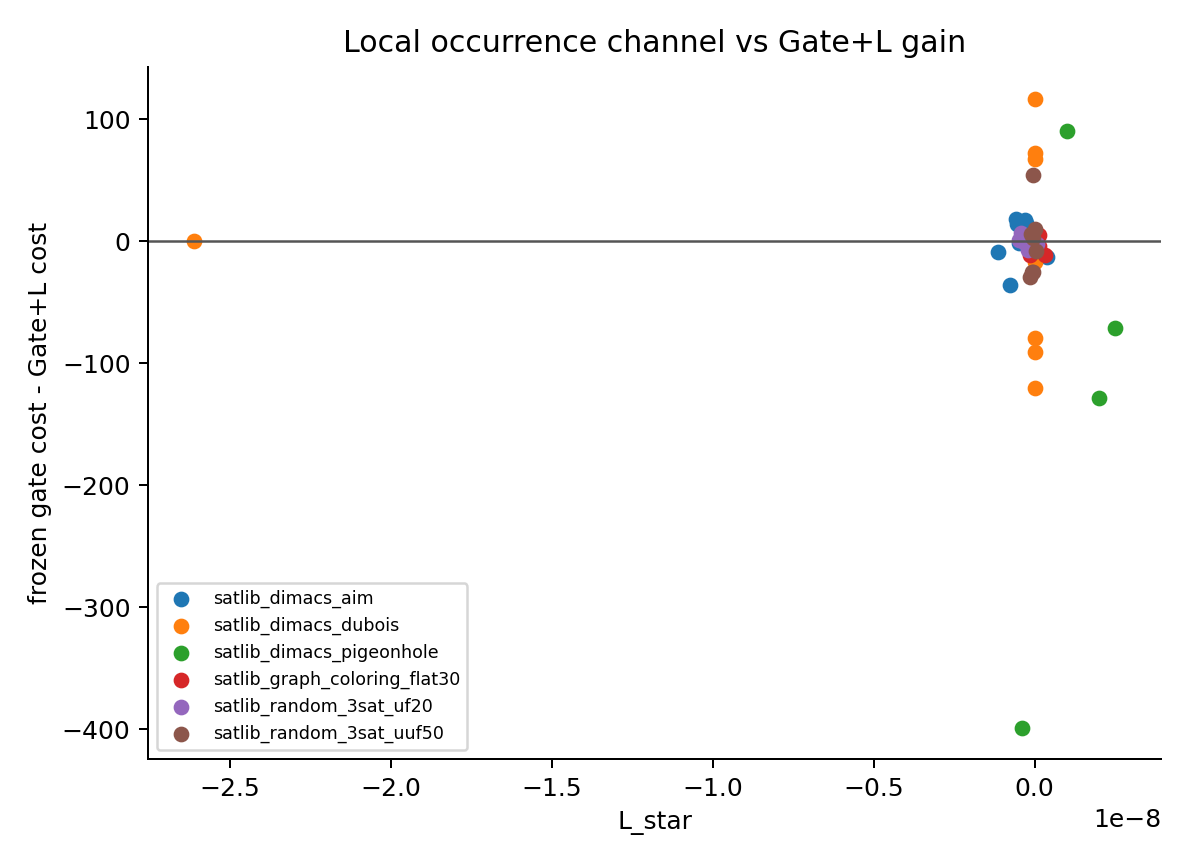
\includegraphics[width=0.90\linewidth]{outputs_paper73_local_occurrence_execution/fig4_lstar_vs_gate_gain.png}
\caption{Gate gain against $\Lstar$ on the test split. The local occurrence
coordinate does not produce a robust positive execution signal under the frozen
protocol.}
\end{figure}

\section{Interpretation}

The execution result is
\[
  \boxed{\texttt{no\_minimum\_support}}.
\]
The preregistered Local Occurrence Hypothesis was tested under the predefined
protocol and was not supported.

This negative result should be read narrowly. It does not show that local SAT
structure is irrelevant, and it does not reinterpret the Paper-72 protocol.
Rather, it shows that the specific frozen occurrence/degree residual channel
defined in Paper 72 did not provide robust practical decision utility under the
first external execution.

\begin{center}
\fbox{\begin{minipage}{0.92\linewidth}
\textbf{Central execution observation.}
The near-collinearity of the residualized occurrence and degree channels after
calibration-only residualization rendered $\Lstar$ effectively inactive in this
execution.
\end{minipage}}
\end{center}

The detailed numbers in the frozen feature output confirm this observation.
The maximum absolute difference between $O_{\rm raw}$ and $D_{\rm raw}$ was
$2.08\times10^{-10}$, and the maximum absolute difference between $O_{\rm res}$
and $D_{\rm res}$ was $1.14\times10^{-10}$. Consequently $\Lstar$ was
effectively zero (standard deviation $3.53\times10^{-9}$), and $\Glocal$
remained practically indistinguishable from the frozen gate (maximum absolute
deviation $6.19\times10^{-10}$). In this execution, the predeclared local
channel therefore did not become an additional operative branching signal.

This sharpens the scientific reading of the negative result. The
\texttt{no\_minimum\_support} classification is correct under the frozen
criteria, but the execution should not be read as a decisive test of all
possible occurrence/degree local-channel ideas. It tested the specific
Paper-72 operational construction, and that construction collapsed onto a
nearly redundant pair of channel measurements in this SATLIB implementation.
Thus the frozen hypothesis was tested faithfully, but the added channel did
not carry independent signal in the executed form.

Two outcome-level observations are especially important. First, Gate+L did not
robustly beat the frozen v1.7 gate or score-with-R. Second, Gate+L did not
survive the shuffled-$L$ null. Together, these outcomes rule out minimum support
under the predeclared criteria. The negative comparison against MOMS further
indicates that classical decision-local short-clause pressure remains a stronger
SAT branching signal in this benchmark.

\section{Limitations}

This paper reports one frozen execution, not a new search for better SAT
features. The benchmark is SATLIB-based and family-balanced only at the
selected-family level. The transparent solver backend is useful for auditability
but is not a substitute for highly optimized modern CDCL implementations.

No new hypothesis is introduced here. Any future local-channel refinement would
require a new preregistered protocol and a new execution paper.

\section{Reproducibility}

The experiment folder is:
\begin{verbatim}
experiments/local_occurrence_execution_paper73/
\end{verbatim}

The repository is:
\[
\text{\url{https://github.com/Chris4081/structural-selection-principle}}.
\]

The preregistered Paper-72 protocol artifact used by this execution is:
\begin{verbatim}
../local_occurrence_hypothesis_paper72/
outputs_paper72_local_occurrence_protocol/paper72_protocol.json
\end{verbatim}

Raw SATLIB CNF files are intentionally not committed. They must be staged from
the original SATLIB source and verified against the SHA256 manifest before any
solver execution:
\begin{verbatim}
python3 download_satlib_paper73.py --allow-insecure-ssl
python3 local_occurrence_execution_paper73.py --validate-only
\end{verbatim}
The insecure-TLS flag records provenance metadata only and does not affect
gate parameters, residualization, calibration, policies, budgets, or
interpretation criteria.

The frozen execution is reproduced by:
\begin{verbatim}
python3 local_occurrence_execution_paper73.py
\end{verbatim}

Primary outputs are written under:
\begin{verbatim}
outputs_paper73_local_occurrence_execution/
\end{verbatim}
and include:
\begin{itemize}
  \item \texttt{paper73\_dataset\_validation.json},
  \item \texttt{paper73\_summary.json},
  \item \texttt{paper73\_solve\_records.csv},
  \item \texttt{paper73\_gate\_l\_features.csv},
  \item \texttt{paper73\_gate\_l\_comparisons.csv},
  \item \texttt{paper73\_policy\_summary.csv},
  \item \texttt{paper73\_family\_results.csv},
  \item \texttt{paper73\_shuffled\_l\_null.csv}.
\end{itemize}

The committed CSV/JSON files and figures are derived artifacts. They do not
contain raw DIMACS clauses and do not redistribute SATLIB benchmark instances.

\section{Conclusion}

Paper 73 completes the first execution of the Local Occurrence Hypothesis
defined in Paper 72. The dataset gatekeeper passed, the solver pipeline ran,
and the output is reproducible from the committed code, manifest, and derived
CSV/JSON files. Under the preregistered interpretation rule, the hypothesis
receives \texttt{no\_minimum\_support}.

The scientific value of the result is methodological: the MAAT Gate Challenge
cycle generated a concrete hypothesis, froze it, executed it externally, and
accepted the negative outcome without modifying the preregistered hypothesis.

\begin{thebibliography}{9}

\bibitem{satlib}
H.~H. Hoos and T.~Stützle,
\emph{SATLIB --- Benchmark Problems}.
Public benchmark page, accessed 2026.
\url{https://www.cs.ubc.ca/~hoos/SATLIB/benchm.html}.

\bibitem{chaff}
M.~W. Moskewicz, C.~F. Madigan, Y.~Zhao, L.~Zhang, and S.~Malik,
``Chaff: Engineering an Efficient SAT Solver,''
in \emph{Proceedings of the 38th Design Automation Conference}, 2001.

\bibitem{jeroslow-wang}
R.~G. Jeroslow and J.~Wang,
``Solving propositional satisfiability problems,''
\emph{Annals of Mathematics and Artificial Intelligence}, 1, 167--187, 1990.

\bibitem{seriesii}
C.~Krieg,
\emph{MAAT Research Series II --- Gate Challenge Cycle I}.
Zenodo, 2026.
\url{https://doi.org/10.5281/zenodo.21062386}.

\end{thebibliography}

\end{document}
